%!TEX root = ../main.tex
\chapter{Methodology}\label{chapter:methodology}
In this chapter we will give overview of our system design and work flow.
First, in~\autoref{sec:Terminology}, we will give technical descriptions of terms we will be using to describe our work flow.
In~\autoref{sec:Work Flow}, we will describe the overall procedure of our research work.
\section{Terminology}
\label{sec:Terminology}
In this section we give a detailed description of different terms we will be using through out the report.
\subsection{Behavioral Profile}
\label{sub:Behavioral Profile}
\citeauthor{bayer} define \textbf{behavioral profile} as, ``the abstraction of a program's execution trace that provides information on the OS objects that the program operated on, along with the operations''.
OS Object refers to resource type such as file, registry or section, that could be modified or queried with the system calls.
System calls consisted of Windows NT, native API and the Windows API functions.
A program uses Windows API and native API functions to communicate with the Windows system such as creating a file or deleting a registry.\\

The behavioral profile was based on the execution traces of programs irrespective of order execution as reordering system calls could be done without changing the semantics of program~\cite[]{bayer}.
It consisted of a list of different operations operated on the different OS objects during the execution of binary.
The system calls that had same purpose as resultant output but different calling API name were generalized under single name---\emph{NtCreateProcess} and \emph{NtCreateProcessEx} would be generalized as, \emph{`create'} OS Operation for, \emph{`porcess'} OS object~\cite[]{bayer}.\\
\subsubsection{OS Objects}
\label{ssub:OS Objects}
OS Object were primarily the resource that were created, delete, modified during the program execution.
\citeauthor{bayer} define \emph{OS Objects} as:
\begin{lstlisting}[numbers=none]
OS Object ::= (type, object-name)
type ::= file|registry|process|job|
       network|thread|section|
       driver|sync|service|random|
       time|info
\end{lstlisting}
An OS Object consists of its type and object-name.
The type of OS Object are file, registry, process, job, network, thread, section, driver, sync, service, random, time, and info.
An object-name is the name of the OS object.
For an instance, \url{`c:\\ntlos.exe'} is an object-name for object type \emph{file}.

\subsubsection{OS Operations}
\label{ssub:OS Operations}
Broadly, OS Operation is the generalization of a system call.
\citeauthor{bayer} define \emph{OS Operations} as:
\begin{lstlisting}[numbers=none]
OS operation ::= (operation-name,
                opeartion-attributes?,
                successful?)
\end{lstlisting}
An OS operation object consists of name of the operation, any additional attributes, and the status of the operation whether it was successful or not.\\
A snippet of behavioral profile is shown in~\autoref{lst:bpsample} with sample of operations executed on OS Objects file, registry, and section.
\begin{lstlisting}[numbers=none,language=TeX,caption={Behvaioral Profile sample}, label={lst:bpsample}]
  op|file|`C:\\Program Files\\Common Files\\sumbh.exe'
   create:1
   open:1
   query:1
   write:1

  op|registry|`HKLM\\SOFTWARE\\CLASSES\\CLSID\\{00021401-000000000046}'
   open:1
   query:1
   query_value(''):1
   query_value('InprocServer32'):0

  op|section|`BaseNamedObjects\\MSCTF.MarshalInterface.FileMap.ELE.B.FLKMG'
   create:1
   map:1
   mem_read:1
   mem_write:1
\end{lstlisting}
To explain the behavioral profile shown in~\autoref{lst:bpsample}, \textit{`create'} operation for file OS object \url{`C:\\Program Files\\Common Files\\sumbh.exe'} was successful with success value 1, whereas \textit{`query\_value'} operation with operation-attribute value \emph{'InprocServer32'} for registry OS Object \url{`HKLM\\SOFTWARE\\CLASSES\\CLSID\\{00021401-000000000046}'} failed with success value 0. % chktex-file 8
\\

We had the ``behavioral profiles'' of the malware samples that we used to create new database which is described in~\autoref{sec:Creation of Database}.
Informations from \emph{OS Objects} and \emph{Operations} were used to extract resource activities (execution traces) of the malware (program).
% recreate the database of all the malware (program) samples and its resource activities (execution traces).

\subsection{Resource Type and Activities}
\label{sub:Resource Types and Activities}
As discussed before in~\autoref{ssub:OS Objects}, an OS Object, are representation of resource types.
For our research, we considered following 8 resource types into consideration, that could best determine the behavioral interference between malware.
These resource types are the most common resource that malware modifies in order to infect the system and disable security services.
We will give a short description of each resource type according to Microsoft Developers Network documentation~\cite[MSDN]{msdn}.
\subsubsection{File}
\label{ssub:File}
A \emph{file} is a means of storing resourceful information which can be retrieved or modified in future.
File objects function as the logical interface between kernel and user-mode processes and the file data that resides on the physical disk.
It not only holds the data written on the file but also a set of attributes maintained by the kernel for system purposes such as \emph{File name, Current byte offset, Share mode, I/O mode}~\cite[]{msfile}.\\
File type in the behavioral profile encompasses not only general file, but named pipe and mailslot resources.
% File is an important resource type for us to focus as our hypothesis for research is that malware of certain family creates or deletes a certain file to infect a system and this also could be used by malware of another family to remove its nemesis from system.
File is an important resource type as many malware creates or deletes file in order to infect the system or remove another malware from the system.
These file activities will be important behavior to find the interference between malware families.
\subsubsection{Registry}
\label{ssub:Registry}
A \emph{Registry} is a database defined by a system where different applications and system components store and retrieve data such as configurations settings for its use.
The data stored in the registry varies according to the version of Microsoft Windows.
Application performs the basic add, modify, retrieve, or delete operation in the registry through the registry API~\cite[]{msregistry}.\\
% We take the registry keys associated with the malware into consideration for experiment as it provides vital information on the behavior of a malware sample.
% Malware with same family might have similar registry key activity and also malware from different family might look for the particular registry key in the system in order to detect the presence of another family.
Registry keys provide vital information on malware type and behavior as we have seen in~\autoref{sec:Malware Types and Families} that different malware families create different registry keys when they infect a system.
Malware from same family modify specific registry key, which is used to detect their presence.
\subsubsection{Service}
\label{ssub:Service}
A \emph{Service} is a computer program that operates in system background, similar to UNIX daemon~\cite[]{servicedef}.
A \emph{service} can be started at system boot through the Service Control Panel, or an application can also use service functions such as \emph{StartService, OpenService, DeleteService} to configure services.
However, it must conform to the interface rules of Service Control Manager (SCM)~\cite[]{msservice}.\\
Malware can stop other services related to security or other malware, create a new service, or hook itself into autostart services.
These service related activity are thus interesting to study malware behavior and interaction with other malware.
\subsubsection{Section}
\label{ssub:Section}
A \emph{section} object is sharable memory which is used by process to share its memory address space (memory sections) with other processes.
It is also used by process to map a file into its memory address space~\cite[]{mssection}.\\
In case of behavioral profile, it broadly represents memory mapped files---file with content in virtual memory, enabling application and multiple processes to modify the file by reading and writing directly to the memory~\cite[]{memmapfile}.
\subsubsection{Process}
\label{ssub:Process}
A binary can spawn one or more \emph{processes}.
A \emph{process} is simply an instance of a computer program being executed that consists of instructions and current activity of program~\cite[]{msprocess}.\\
Malware trying to detect and kill the process created by another malware is interesting case of behavioral interference.
% Malware constantly looks for creation of some utility processes, such as \emph{Task Manager} or \emph{Virus Removal Tools}, and shuts it down, as soon as the process starts.
% Similar behavior of malware, to check for process created explicitly by other malware samples, will be a proof for behavioral interference between malware families.
\subsubsection{Job}
\label{ssub:Job}
A \emph{Job} object makes grouping of process as single unit to manage possible.
It can be named and shared securely to control attributes of processes grouped together and operation on a job makes the affect on all the process in its group~\cite[]{msjob}.
\subsubsection{Sync}
\label{ssub:Sync}
A \emph{sync object} is used to coordinate the execution of multiple threads as more than one process could share the handle of single synchronization object which helps for the interprocess synchronization between these processes~\cite[]{mssync}.\\
The sync object type covers all the synchronization activities.
\cite[]{mssync}.
\subsubsection{Driver}
\label{ssub:Driver}
A \emph{device driver } is a program that is associated with certain device for its operation and control. It is used as an software interface to communicate between the hardware device and the operating system and other software~\cite[Device Driver]{devicedriver} \\
Windows represent devices with device objects, and one device could be represented by more than one device objects. All operation on device is conducted via device object~\cite[]{msdevice}.\\
We capture those loading and unloading of Windows Device Driver recorded in the behavioral profile.\\

\textbf{Resource activities} in our work refers to operations, such as \emph{create, delete, modify, or access}, performed by a malware (program), on the resource types \emph{File, Registry, Service, Section, Process, Job, Sync, or Driver}, during its execution.
\textbf{Resource name} is same as object-name in \emph{OS-Objects}[\autoref{ssub:OS Objects}]---name of the resource created, modified, deleted, or accessed.
We use resource activities of malware samples to select the malware candidates that could exhibit behavioral interference [\autoref{sec:Initial Experiment}].
Further, resource activities related to malware were represented as \emph{``words''} related to \emph{``document''} (malware) to create a text corpora for document clustering [\autoref{sec:Document Clustering}].
% We will illustrate the implementation of resource activities in malware clustering in~\autoref{sec:Document Clustering}.
We describe the terms \emph{``words''}, \emph{``document''}, and \emph{``corpora''} in~\autoref{sub:Words, Document, Corpora}.
\subsection{Words, Document, Corpora}
\label{sub:Words, Document, Corpora}
% We have already discussed about using \emph{LDA} for clustering the malware in~\autoref{sec:Malware Clustering}, and what resource activities are in~\autoref{sub:Resource Types and Activities}.
In this section, we describe the terms \emph{``words''}, \emph{``document''}, and \emph{``corpora''} and how we associate, malware samples and resource activities, with those terms in our work.
The terms will be used extensively when describing clustering [\autoref{ssub:Latent Dirichlet Allocation}] and its implementation [\autoref{sec:Document Clustering}].
\subsubsection{Words}
\label{ssub:Words}
In their work,~\citeauthor{Blei}, describe word as, `A \emph{word} is a basic unit of discrete data, defined to be item from a vocabulary indexed by $\{1,\ldots,V\}$''~\cite[]{Blei}.\\
We represent a single resource activity of a malware as single word.
For an instance, a file creation activity will be a single distinct word and a file deletion activity will be another distinct word.
Same resource activity---with same resource type, resource name and operations---will be considered as repetition of same word.
For example, multiple registry keys created with same name by same or different malware.
\subsubsection{Document}
According to~\citeauthor{Blei}, ``a \emph{document} is a sequence of $N$ words denoted by $\textbf{w} = (w_1,w_2,\ldots,w_N)$, where $w_N$ is the $n$th word in the sequence''~\cite[]{Blei}.\\
A single malware sample will be represented as a single document and all the resource activities related to that malware will be the words in that document.
\label{ssub:Document}
\subsubsection{Corpora}
\label{ssub:Corpora}
``A \emph{corpus} is a collection of $M$ documents denoted by $D = \{w_1,w_2,\ldots,w_M\}$''~\cite[]{Blei}.\\
The total resource activities (words) related to all the malware samples (documents), in our dataset, will be our corpus.\\

\section{Work Flow}
\label{sec:Work Flow}
% In previous section, we described different terms we use in our work to help reader properly understand the usage of those terms.
In this section we outline an overview of our work flow.
Figure~\ref{fig:bigpicture} depicts the overall structure of of our system.
We describe about the old database that we had access to and the need for the creation of new database in~\autoref{sub:Database}.
We create reverse index from the database and use heuristics to select candidate pair which is described in~\autoref{sub:Reverse Indexing} and~\autoref{sub:Heuristics} respectively.
To lower the number of candidate pair and find malware pair belonging to different families, we cluster the malware based on their behavioral profile as described in~\autoref{sub:Clustering}.
The candidate pair selection based on clustering is described in~\autoref{sub:Candidate Selection}.
In~\autoref{sub:Running the Candidate} and~\autoref{sub:Result Analysis}, we describe running the candidate pair and analyzing the result respectively.
\subsection{Database}
\label{sub:Database}
We required resource activities of the malware samples to process and find malware with behavioral interference.
For every binary submitted to Anubis for analysis, it executes the binary inside the emulated environment and keeps track of operating system services that are called by the binary.
Anubis does this by keeping the log of all the Windows native system calls and Windows API functions that the binary invokes.
Resource activity such as creating a file or a registry, by the binary with the Windows API functions (\emph{CreateFile, RegCreateKeyEx}), are monitored and recorded.

A portion of sample log file is shown in~\autoref{lst:anubislog}.
In Line 6, \emph{`test.exe'} process was included for the analysis.
Each process is uniquely identified by its page directory base address, which is \emph{0X04660000} in this case. % chktex-file 29
The page directory address ensures that each process has its own virtual memory space.
The page directory address of currently running process is stored in page-directory base register (PDBR)~\cite[]{ttanalyze}.
For the analysis subject \emph{`test.exe'}, we see the log file has record of the loading of \emph{ntdll.dll} (module that contains Windows NT system functions~\cite[]{ntdll}) and \emph{RPCRT4.dll} (Remote Procedural Call API used by Windows application for network and Internet communication~\cite[]{rpcrt}) in Line 5 and Line 13 respectively.
In Line 8--12, we can see the log for different native system calls such as \emph{NtOpenKey, NtDeleteKey,NtCreateKey} related to opening, delete, and creating registry key respectively.
With the log, Anubis generates the report of the analysis (resource activities of the analysis subject), and also keeps the record of the analysis report and the binary file, in the relational database for further record.
We had access to those databases.
The report database has record of resource activities of \emph{File, Registry, Service, Process, and Network} for operations \emph{create, delete, modify, read}.\\

However, the old database was missing the resource activities that were not successful; for an example, failed attempt by malware to delete a file.
For each run, Anubis analyzed malware one at a time in a total new OS environment; so the resources created during one analysis run were not present during the analysis run of another malware.
Because of this, malware trying to detect or delete the resource created by some other malware would be unsuccessful.
A new database with record of such failed attempts was essential.\\

With the log of execution trace and system calls, Anubis also creates the ``behavioral profile'', described in~\autoref{sub:Behavioral Profile}, for the submitted malware sample, which has record of both the successful and failed resource activities.
The ``behavioral profile'' of malware sample was used to get the resource name (object-name)[see~\autoref{ssub:OS Objects}] and operations (operation-name)[see~\autoref{ssub:OS Operations}] with successful or failed status, to create the new database.
The new database was created for the above discussed 8 types of resource (\emph{File, Registry, Service, Section, Job, Process, Job, Sync, and Driver}) and operations were generalized to \emph{modify, read, and delete}.
The implementation is described in~\autoref{sec:Creation of Database}.
\begin{lstlisting}[float,floatplacement=ht,language=TeX,caption={Snippet of Anubis Log},label={lst:anubislog}]
 Anubis Logfile Version: 1.1
 Starting Anubis at 02/04/16, 02:22:23 UTC.
 Logging all function calls: 0
 00:00:18.389876 [ANALYSIS_INFORMATION]: X X Added all of ntdll.dll's exported functions to the function Addresses Map.
 00:00:18.390846 [ANALYSIS_INFORMATION]: X X ntdll.dll was loaded.
 00:00:18.391247 [ANALYSIS_COORDINATOR]: X X Going to include test.exe with PDB 0x04660000 in the analysis.
 00:00:45.363931 [ANALYSIS_COORDINATOR]: "test.exe" 0 1 Event 'First instruction of the process' happened.
 00:00:45.365954 [FUNCTION_COORDINATOR]: "test.exe" 0 1 Added callback for function NtOpenKey (7C90D5B0)
 00:00:45.366673 [FUNCTION_COORDINATOR]: "test.exe" 0 1 Added callback for function NtDeleteKey (7C90D230)
 00:00:45.367363 [FUNCTION_COORDINATOR]: "test.exe" 0 1 Added callback for function NtCreateKey (7C90D0D0)
 00:00:45.555742 [ANALYSIS_INFORMATION]: "test.exe" 0 1 Added all of RPCRT4.dll's exported functions to the function Addresses Map.
 00:00:45.556358 [ANALYSIS_INFORMATION]: "test.exe" 0 1 RPCRT4.dll was loaded.
\end{lstlisting}
\subsection{Reverse Indexing}
\label{sub:Reverse Indexing}
After we created the database, we created reverse index of the resource activities.
The database had all the resource activities (failed and success) of the resource types: such as file created, file deleted, registry modified, registry accessed and so on.
We mapped `resource name', with all the malware, that had operations on that `resource name'.
For instance, we mapped the resource name of the \emph{files}, with all the malware that modified it.
Same reverse index was generated for read and delete operations, and for other resource types, \emph{registry}, \emph{Section}, and others.
With the reverse index, for each resource, we have a list of all the malware that modified, accessed, or deleted that resource.
We used the reverse index in our heuristics to select candidate malware pairs.
\subsection{Heuristics}
\label{sub:Heuristics}
We mapped reverse indexes, based on common resource name, to get malware set, say set \emph{`A'}, that created a resource \emph{`r'} with another malware set, say set \emph{`B'}, that tried to delete or read the same resource \emph{`r'}.
As described in~\autoref{sec:Malware Types and Families}, malware families have different ways of infecting and taking control of system, peculiar to themselves.
One can detect the presence of malware in the system, by checking the presence of unique resource (files, registries, and others) associated with that malware, in the system.
Thus, when a malware tries to access or delete some resource created by another malware (with a failed attempt because each malware was analyzed by Anubis in new OS environment), that activity is interesting for our candidate selection.\\

We selected malware sample from each of those set \emph{`A'} and \emph{`B'}, to get a candidate pair, with interference corresponding to the resource \emph{`r'}.
For an instance, if $(x_1,x_2)$ belonged to set `A' and $(y_1,y_2)$ belonged to set `B', then the candidate pairs related to resource `r' are: $(x_1,y_1)$, $(x_2,y_2)$, $(x_2,y_1)$, and $(x_2,y_2)$.
With initial testing, we found that a single resource name was created by tens of thousands of malware and being accessed by tens of thousands of another malware.
Large number of candidate pair would be generated even for single resource with this approach.
We had to lower the number of candidate pair to get substantial number that we can test for behavioral interference.
Also, the candidate pair were chosen only based on common resource, and did not represent different families.
We use clustering of malware based on the similarity of behavioral profile to address these problems.
\subsection{Clustering}
\label{sub:Clustering}
Malware variants belonging to same family, will have similar behavior pattern (code semantics) despite of code obfuscation.
With clustering, we group such similar behaving malware into same cluster (family).

Many previous research based on malware clustering were done for small number of malware samples [see~\autoref{sec:Malware Clustering}].
We needed an approach to cluster millions of malware samples.
We modeled malware clustering to \emph{document clustering} and used \emph{LDA} for its low memory footprint, $O(\#words\times \#clusters)$, compared to \emph{tf-idf}, $O(\#documents \times \#words)$.
We use \emph{Gensim}---python library---to implement the document clustering.
\subsubsection{Latent Dirichlet Allocation}
\label{ssub:Latent Dirichlet Allocation}
%TODO: write about LDA
% -- write more about LDA --\\
A single resource activity---such as `file read', `registry delete' or `service modify'---would count as single \emph{`word'}.
All such resource activities of a single malware sample, is the total `words' in the single document (malware).
We created the corpus for document clustering with all the resource activities of all the malware dataset.
We gave each resource type, operation name, and resource name a unique numeric code to represent the resource activity as a word.
The number coding is given in~\autoref{lbl:numericode}
\begin{lstlisting}[numbers=none,language=python,caption={Numeric codes given to resource and operation},label={lbl:numericode}]
  RESOURCE_CODE    = {"file" : "1", "registry" : "2", "section" : "3", "service" : "4", "driver" : "5", "sync" : "6", "process" : "7", "job" : "8"}
  OPERATION_CODE   = {"access" : "1", "delete" : "2", "modify" : "3"}
\end{lstlisting}

A file delete activity of filename, \textit{`c:\textbackslash\textbackslash{}gbot.exe'}, with \textit{file\_name\_id}, ``4986'' in our database, by some malware ``A'', would be represented as single word \emph{``1\_2\_4986''}.
With the corpus created, we use \emph{Gensim} (python library) to perform the document clustering.
\subsubsection{Gensim}
\label{ssub:Gensim}
\emph{``Gensim''}~\cite[]{gensim} is an efficient python library.
We preferred using it because of its simplicity, well documented API, and ability to work on large corpus.
We use the \emph{multicore} models of \emph{Gensim} for scalability as it utilizes the multi cores processor of the machine efficiently with parallelization making the clustering process faster~\cite[]{ldamulticore}.
The document can be fed sequentially to the algorithm making it possible to input large number of documents with the help of iterator.
% The maximum size of our corpus was 81 Gigabytes.
% Some of the benefits of using the \emph{ldamulticore} model were~\cite[]{ldamulticore}:
% \begin{itemize}
% \item The model utilized the multi cores processor of the machine efficiently with parallelization making the clustering process faster.
% \item The training algorithm is streamed and we could feed the input documents sequentially even for large data.
% \item The training algorithm runs in constant memory with respect to number of documents.
% This made possible for us to process corpora that was larger than the memory size of our machine, as size of training corpus did not affect the memory footprint.

% \end{itemize}
\subsection{Candidate Selection}
\label{sub:Candidate Selection}
In this section, we illustrate the candidate pair selection algorithm based on malware clustering.
We select the candidate pair in such a way that two malware associated by an interesting resource (resource created by one malware sample and tried to delete/access with failure by another), fall in different cluster.

Let, \emph{R}, be a set of candidate resources such that each resource ``r'' in \emph{R} have some malware set that create it (say set $A_r$) and some other set of malware that try to (unsuccessfully) access/delete it (say set $B_r$).
We combine all such sets $A_r$ and $B_r$ corresponding to ``r'' in \emph{R} to sets \emph{A} and \emph{B}, respectively.
We combine sets `A' and `B' and cluster them to cluster ids $[c_1,c_2,\ldots.\ c_n]$ (\emph{n} is number of family) such that any malware sample \emph{x} in (\emph{A} union \emph{B}) can be tagged/mapped to cluster id $C(x)$, where $C(x)$ belongs to $[c_1, c_2, \ldots c_n]$.
After the clustering is done we select candidate as shown in algorithm~\autoref{alg:Candidate Selection}.
\begin{algorithm}[ht]
\caption{Candidate Selection}
\label{alg:Candidate Selection}
\begin{algorithmic}[1]
    \State$R$   = Set of all interesting resource
    \State$A_r$ = Set of malware that creates a particular resource `r'
    \State$B_r$ = Set of malware that delete/access (failed) particular resource `r'
    \State$B_r$ = Set of malware that delete/access (failed) particular resource `r'
    \State$N$   = Maximum number of families to consider
    \State$E$   = Set of all probable candidate
    \Function{C}{$j$}
      \State\ $c_j =$ cluster id that malware $j$ belongs to
      \State\ \Return\ $c_j$
    \EndFunction\
    \ForAll{$r \in R$}
      \If{|$C(x_r): x \in A_r| > N \lor |C(y_r): y \in B_r| > N$}
        \State\ \textbf{continue}
      \EndIf\
      \ForAll{$(x_r,y_r) \in A_r \times B_r$}
        \If{$C(x_r) \neq C(y_r)$}
          \State$E\gets (x_r, y_r)$
        \EndIf\
      \EndFor\
    \EndFor\
  \end{algorithmic}
\end{algorithm}

In algorithm~\autoref{alg:Candidate Selection}, we define a function $C(j)$ in line 7--10 which returns the cluster id of given malware $j$.
In line 11--20, for all resource $r$ in set $R$, we first check if the number of create or access/delete families associated with the resource $r$ is greater than $N$.
We choose $N$ accordingly to filter resource associated with too many families.
If true, we simply discard it, as resource modified/deleted by too many families is less interesting.
If false, for every possible malware pair between the create set $A$ and access/delete set $B$, say $(x_r,y_r)$, we populate our experiment set $E$, such that $x_r$ and $y_r$ belong to different family.
The final experiment set \emph{E} is a set of such $(x_r, y_r)$ for all resources \emph{r} in \emph{R}.

We decrease the number of candidate pairs with this approach, as we no more take into consideration all the possible candidate pair from tens of thousands of malware sample associated with resource, but select candidate pairs based on cluster those malware sample belongs to.
For an example, let $r_1$ be the resource which was created by malware samples $x_1,x_2,x_3$ and was tried to delete with failure by malware samples $y_1, y_2, y_3$.
Let, $x_1,x_2,y_1,y_2$ malware samples belong to cluster $c_1$, $x_3$ malware sample belongs to cluster $c_2$, and $y_3$ malware sample belongs to cluster $c_3$.
With previous heuristics, the total candidate pairs would be all possible pairs from the cross product of both set such as $(x_1,y_1), (x_1,y_2), (x_1,y_3),\ldots ,(x_3, y_3)$.
With candidate selection algorithm, we would only get two probable candidate pairs corresponding to resource $r_1$: $(x_1,y_3)$ and $(x_3,y_3)$, such that both malware in the pair belong to different family.
\subsection{Running the Candidate}
\label{sub:Running the Candidate}
Our chosen dynamic analysis system [see \autoref{sub:Anubis}], \emph{Anubis}, analyzes only one binary at a time.
We used the fact that Windows PE executable loader works fine even with extraneous concatenated data at the end of valid executable file.
We created \emph{`packer'} and \emph{`unpacker'}, based on the above fact, to execute both malware of a candidate pair, packed together as single binary, with time interval in between two execution.
The \textbf{unpacker} is a self reading dropper binary.
With \textbf{packer}, we append binary of the candidate pair, to the back of \emph{unpacker} binary, one after another in sequence.
Followed by the binary, meta-information, such as size of both binary and preferred time delay, was appended to the end of the \emph{unpacker}.
We analyze the packed \emph{unpacker} binary in the \emph{Anubis}.
When executed, the \emph{unpacker}, would read itself from the behind to get the meta-information, and recreate the packed binaries, and drop them inside the \emph{Anubis} OS environment.
After both the binaries are dropped, it execute the first binary, waits for specified time delay, and then runs another binary.
The sequence of the binary execution is: candidate malware that creates the resource first, followed by candidate malware that tried to access/delete the resource with failure.
In the end, both the binary runs in the \emph{Anubis}, and we analyze the Anubis report.
In~\autoref{sec:packerunpacker}, we implement the \emph{packer} and \emph{unpacker}.
\subsection{Result Analysis}
\label{sub:Result Analysis}
A binary submitted to Anubis is renamed into \emph{`sample.exe`}, and is considered as the primary analysis subject.
% All the binaries created and executed, after the execution of primary analysis subject, is tracked for its malicious activities.
All the binaries created and executed by the primary analysis subject, after its execution, is also tracked for its resource activities.
% \emph{Anubis}, generates result of analysis as \emph{Extensible Markup Language} (XML) format.
% The XML report has the resource activities of each binaries presented under different XML node.\\
% We analyze the activities of two malware binary, candidate pair, that gets dropped by unpacker and executed.
We analyze the resource activities of our candidate pair and any other process started by them.
We are interested in `access/delete' activity of the `resource', based on which the candidate pair was chosen---`resource' created successfully by one malware, and failed attempt to access/delete the same resource by another.
Any successful access/delete of that resource (files or registries or others) will be the change in behavior of one malware caused by the presence of another malware.

\begin{figure}[htbp]
  \centering
  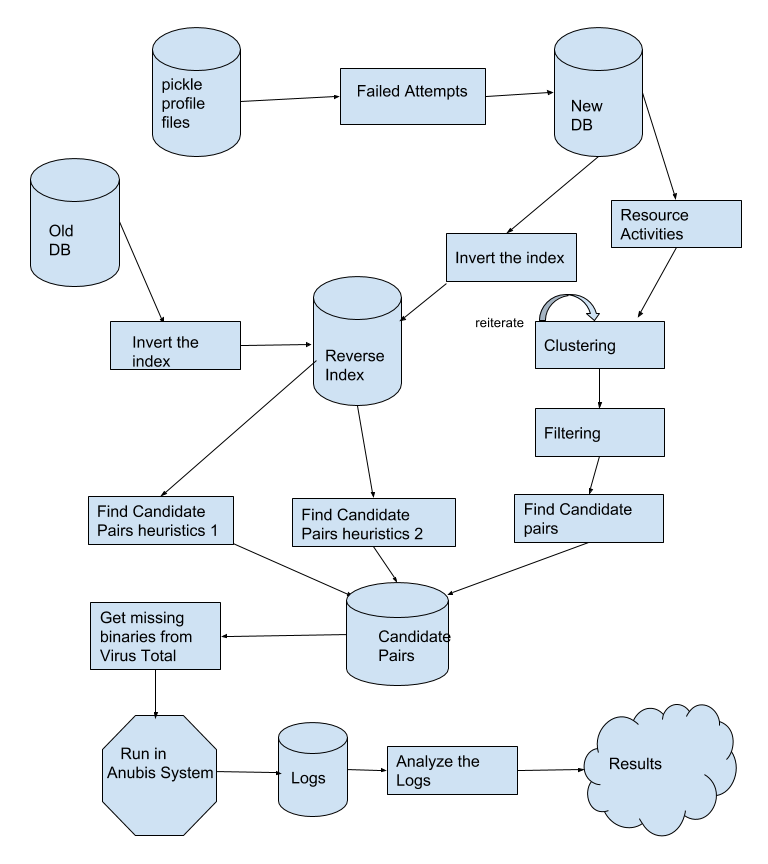
\includegraphics[scale=0.47]{figures/bigpicture.png}
  \caption[Big Picture]{Overview of the research and experiment}\label{fig:bigpicture}
\end{figure}

\section{Summary}
\label{sec:ssummary}
In this chapter, we described different terms used in our work in details and also gave an overview of our work flow.
In next chapter, we will show how we implemented the work flow in our system.
